\chapter{Konzeption}
\label{chap:konzeption}
Das im Rahmen dieser Arbeit entwickelte verteilte Echtzeit-3D-Renderingsystem hat den Namen \textit{Osiris}. Der Name bedeutet \textit{Online SIRIS}, da der WebGL-Renderer auf der einen Seite ohne das SIRIS-Backend nicht wie erwartet funktionieren würde und er zudem einige der Möglichkeiten von SIRIS online über den Browser verfügbar macht.
\begin{figure}
\centering
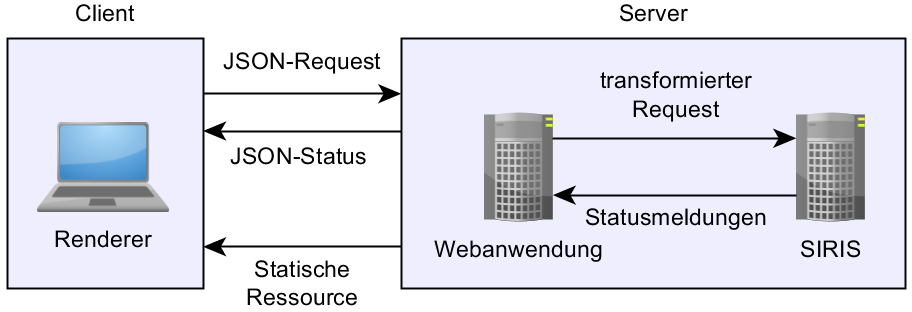
\includegraphics[width=\textwidth]{bilder/structure.png}
\caption{Prinzipielle Sytemstruktur}
\label{fig:structure}
\end{figure}
Osiris besteht aus einem WebGL-Renderer und einem Webserver, der statische Ressourcen bereit stellt und die Kommunikation über eine WebSocketverbindung mit dem SIRIS-Backend steuert. Auf dem Webserver wird auch SIRIS inklusive der angebundenen Physikengine ausgeführt. Dieses Setup überlässt dem Client lediglich das Rendern der 3D-Szene, die rechenintensive Physiksimulation findet auf dem Server statt.

Der WebGL-Renderer sowie die Anwendung auf dem Webserver und die Anbindung an SIRIS wurden eigenständig neu implementiert. SIRIS ist auf dem Stand vom 6. Juni 2012, der Quelltext wurde bis auf das Abschalten des leistungszehrenden Benchmarkings nicht verändert.

In der Webanwendung sind mehrere Controller registriert die auf Anfragen reagieren und dem Client bestimmte Informationen bereitstellen. So gibt es jeweils einen Controller für die WebSocket-Kommunikation, Szenen und Shaderprogramme. Dies macht die Organisation der betreffenden Daten auf dem Server für den Client völlig transparent und verringert die Kopplung der funktionalen Komponenten im System. Um den Fokus auf der Anbindung des Renderers an SIRIS zu erhalten und den Komplexitätsgrad der Anwendung nicht zu weit zu steigern wurde auf die Unterstützung mehrerer Anwender verzichtet, da das Play! Framework statuslos ist und für das Vermeiden der Vermischung von Nachrichten eine recht komplexe Verwaltung der unterschiedlichen Anwender hätte implementiert werden müssen. Dies wäre im kurzen Zeitrahmen für diese Arbeit kaum möglich gewesen.

Der Renderer wird mitsamt der HTML-Seite und der für den Stil verantwortlichen CSS-Datei beim Verbinden mit dem Server an den Browser übertragen. Vor der Auslieferung fügt die Webanwendung Informationen über die verfügbaren Szenen und Shaderprogramme in die Webseite ein. Der Benutzer kann nun die darzustellende Szene und das dafür zu benutzende Shaderprogramm wählen woraufhin beides über den Renderer vom Webserver angefordert wird. Dies ermöglicht eine sehr flexible Bereitstellung neuer Szenen und Shaderprogramme.

Im gegenwärtigen Zustand unterstützt der Renderer Beleuchtung mit verschiedenen Lichtquellen und die Texturierung der dargestellten Objekte mit verschiedenen Texture Map-Typen. Über eine Websocketverbindung kommuniziert der Renderer über fest vordefinierte, in JSON enkodierte Nachrichten mit dem Server. Dieser sendet ebenfalls fest vorgegebene JSON-Nachrichten an den Client. JSON ist die Abkürzung für die \textit{JavaScript Object Notation}. Mit dieser lassen sich komplexe, hierarchische Strukturen in Reintextform beschreiben. Tatsächlich ist jede JSON-Nachricht ein valides JavaScript-Objekt. Diese Festlegung etabliert auf beiden Seiten wohldefinierte Kommunikations-APIs, abstrahiert die auf der jeweiligen Seite ablaufenden Prozesse und macht den Unterschied der verwendeten Programmiersprachen völlig transparent. So könnte man den Renderer auch gegen eine völlig andere funktionale Komponente austauschen, solange diese über die gleichen Nachrichten mit dem Server kommuniziert wie der Renderer. Ein kleinerer Nachteil ist, dass JSON nicht die Kompaktheit von binären Datentypen erreicht.

Die Szene wird ebenfalls mittels JSON beschrieben und enthält alle notwendigen Informationen zu ihrer Darstellung und Interaktion und bildet so einen einfachen Szenegraphen ab. Der Wurzelknoten enthält mehrere Gruppenknoten, denen jeweils bestimmte Knotentypen, wie Kameradaten, Informationen über die in der Szene dargestellten 3D-Objekte, Informationen zur Beleuchtung und die zur Manipulation bestimmter Objekte verwendbaren Tasten zugeordnet sind (siehe Abbildung \ref{fig:szenestruktur} und Listing \ref{lst:scenejson}). Durch die Notation in JSON lassen sich so beliebige Szenen sehr flexibel beschreiben wobei der im Rahmen dieser Arbeit entwickelte Renderer auf die Existenz einiger Knoten angewiesen ist.
\lstset{language=JavaScript}
\begin{lstlisting}[caption={JSON-Struktur einer möglichen Szene}, label={lst:scenejson}]
{
  "type": "scene",
  "rootNode": {
    "id": "root",
    "type": "group",
    "children": [
      {
        "id": "options",
        "type": "group",
        "children": [
          {
            "id": "cam",
            "type": "camera",
            "position": {
              ...
            },
              ...
          },
            ...
      },
      {
        "id": "lights",
        "type": "group",
        "children": [
          ...
        ]
      },
      {
        "id": "models",
        "type": "group",
        "children": [
          ...
        ]
      }
    ]
  }
}
\end{lstlisting}
\begin{figure}
\centering
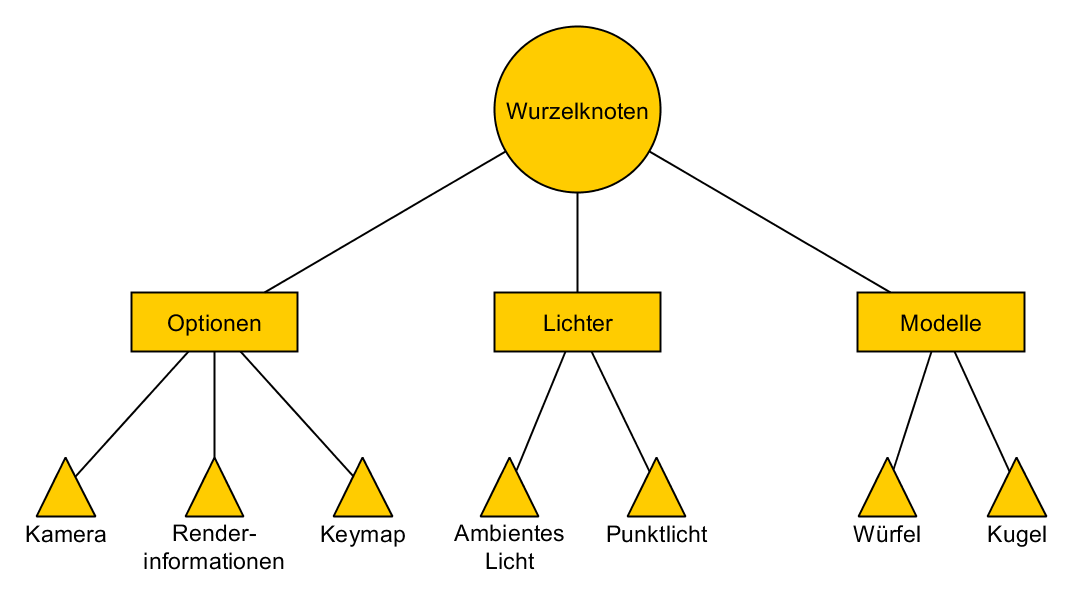
\includegraphics[height=70mm]{bilder/scenestructure.png}
\caption{Beispielstruktur einer Szene}
\label{fig:szenestruktur}
\end{figure}
Auf dem Webserver findet auch die Transformation der JSON-Nachrichten vom Client in ein für SIRIS verständliches Format und umgekehrt von SIRIS an den Client statt. Da sowohl der Renderer als auch die in SIRIS enthaltene Physikengine für jedes Objekt wissen müssen wo es sich wann mit welcher Ausrichtung in der dargestellten Szene befindet, verfügt jeder Objektknoten über eine eigene Transformationsmatrix. Sowohl SIRIS als auch WebGL bilden alle Transformationen in einem Rechtshändigen Koordinatensystem mit den folgenden Vereinbarungen ab:
\begin{itemize}
    \item Die drei Achsen (\textit{x}, \textit{y} und \textit{z}) stehen im rechten Winkel aufeinander.
    \item Die \textit{x}-Achse zeigt nach Osten.
    \item Die \textit{y}-Achse zeigt nach oben in Richtung eines imaginären Himmels.
    \item Die \textit{z}-Achse zeigt nach vorn in Richtung des Betrachters.
\end{itemize}
\begin{figure}
\centering
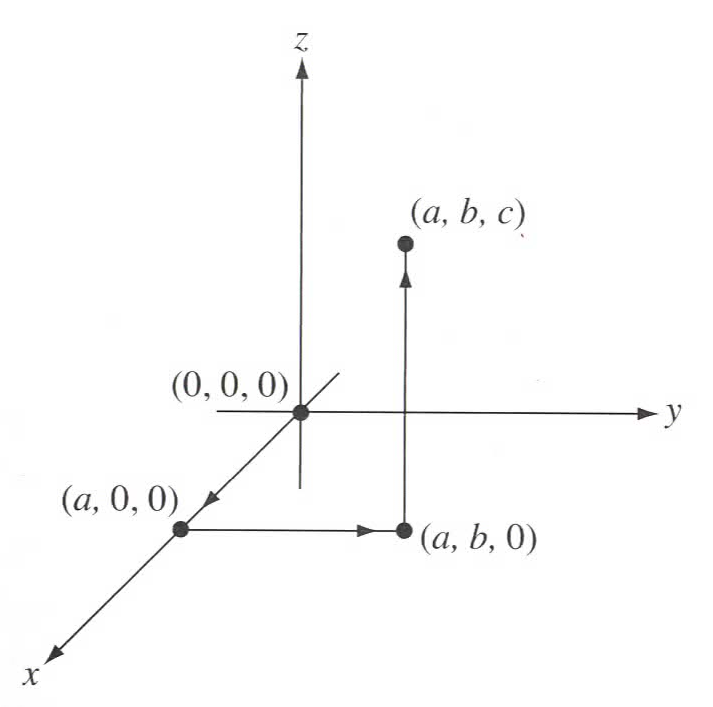
\includegraphics[height=60mm]{bilder/righthandcoordsystem.png}
\caption{Das Rechtshändige Koordinatensystem von JBullet und WebGL}
\label{fig:coordsystem}
\end{figure}